\documentclass[12pt,halfline,a4paper,]{ouparticle}

% Packages I think are necessary for basic Rmarkdown functionality
\usepackage{hyperref}
\usepackage{graphicx}
\usepackage{listings}
\usepackage{color}
\usepackage{fancyvrb}
\usepackage{framed}

% For knitr::kable functionality
\usepackage{booktabs}
\usepackage{longtable}

%% To allow better options for figure placement
%\usepackage{float}

% Packages that are supposedly required by OUP sty file
\usepackage{amssymb, amsmath, geometry, amsfonts, verbatim, endnotes, setspace}

% For code highlighting I think
\DefineVerbatimEnvironment{Highlighting}{Verbatim}{commandchars=\\\{\}}
\definecolor{shadecolor}{RGB}{248,248,248}
\newenvironment{Shaded}{\begin{snugshade}}{\end{snugshade}}
\newcommand{\AlertTok}[1]{\textcolor[rgb]{0.94,0.16,0.16}{#1}}
\newcommand{\AnnotationTok}[1]{\textcolor[rgb]{0.56,0.35,0.01}{\textbf{\textit{#1}}}}
\newcommand{\AttributeTok}[1]{\textcolor[rgb]{0.77,0.63,0.00}{#1}}
\newcommand{\BaseNTok}[1]{\textcolor[rgb]{0.00,0.00,0.81}{#1}}
\newcommand{\BuiltInTok}[1]{#1}
\newcommand{\CharTok}[1]{\textcolor[rgb]{0.31,0.60,0.02}{#1}}
\newcommand{\CommentTok}[1]{\textcolor[rgb]{0.56,0.35,0.01}{\textit{#1}}}
\newcommand{\CommentVarTok}[1]{\textcolor[rgb]{0.56,0.35,0.01}{\textbf{\textit{#1}}}}
\newcommand{\ConstantTok}[1]{\textcolor[rgb]{0.00,0.00,0.00}{#1}}
\newcommand{\ControlFlowTok}[1]{\textcolor[rgb]{0.13,0.29,0.53}{\textbf{#1}}}
\newcommand{\DataTypeTok}[1]{\textcolor[rgb]{0.13,0.29,0.53}{#1}}
\newcommand{\DecValTok}[1]{\textcolor[rgb]{0.00,0.00,0.81}{#1}}
\newcommand{\DocumentationTok}[1]{\textcolor[rgb]{0.56,0.35,0.01}{\textbf{\textit{#1}}}}
\newcommand{\ErrorTok}[1]{\textcolor[rgb]{0.64,0.00,0.00}{\textbf{#1}}}
\newcommand{\ExtensionTok}[1]{#1}
\newcommand{\FloatTok}[1]{\textcolor[rgb]{0.00,0.00,0.81}{#1}}
\newcommand{\FunctionTok}[1]{\textcolor[rgb]{0.00,0.00,0.00}{#1}}
\newcommand{\ImportTok}[1]{#1}
\newcommand{\InformationTok}[1]{\textcolor[rgb]{0.56,0.35,0.01}{\textbf{\textit{#1}}}}
\newcommand{\KeywordTok}[1]{\textcolor[rgb]{0.13,0.29,0.53}{\textbf{#1}}}
\newcommand{\NormalTok}[1]{#1}
\newcommand{\OperatorTok}[1]{\textcolor[rgb]{0.81,0.36,0.00}{\textbf{#1}}}
\newcommand{\OtherTok}[1]{\textcolor[rgb]{0.56,0.35,0.01}{#1}}
\newcommand{\PreprocessorTok}[1]{\textcolor[rgb]{0.56,0.35,0.01}{\textit{#1}}}
\newcommand{\RegionMarkerTok}[1]{#1}
\newcommand{\SpecialCharTok}[1]{\textcolor[rgb]{0.00,0.00,0.00}{#1}}
\newcommand{\SpecialStringTok}[1]{\textcolor[rgb]{0.31,0.60,0.02}{#1}}
\newcommand{\StringTok}[1]{\textcolor[rgb]{0.31,0.60,0.02}{#1}}
\newcommand{\VariableTok}[1]{\textcolor[rgb]{0.00,0.00,0.00}{#1}}
\newcommand{\VerbatimStringTok}[1]{\textcolor[rgb]{0.31,0.60,0.02}{#1}}
\newcommand{\WarningTok}[1]{\textcolor[rgb]{0.56,0.35,0.01}{\textbf{\textit{#1}}}}

% For making Rmarkdown lists
\providecommand{\tightlist}{%
  \setlength{\itemsep}{0pt}\setlength{\parskip}{0pt}}

% Part for setting citation format package: natbib

% Part for setting citation format package: biblatex

% Part for indenting CSL refs
% Pandoc citation processing
% Pandoc header

\begin{document}

\title{POLS 7012 Final Exam}

\author{%
\name{YOUR NAME HERE}\address{University of Georgia}\email{\href{mailto:email@email.email}{email@email.email}}
\and
\name{Joseph T. Ornstein}\address{University of Georgia}\email{\href{mailto:jornstein@uga.edu}{jornstein@uga.edu}}
}

\abstract{}

\date{December 07, 2020}

\keywords{}

\maketitle



\hypertarget{introduction}{%
\section{Introduction}\label{introduction}}

In this paper, we will replicate the results from ``Civic Honesty Around
the Globe'' (Cohn et al. 2019). Anything I call an ``extra challenge''
is available for the intrepid among you, but is not required.

To submit your final exam, knit this \texttt{.Rmd} to a PDF and post the
PDF to eLC.

\hypertarget{data}{%
\section{Data}\label{data}}

Replication files are available
\href{https://dataverse.harvard.edu/dataverse/honesty}{here}, and I have
already downloaded them into the \texttt{data/} folder. Let's load the
behavioral data.

\begin{Shaded}
\begin{Highlighting}[]
\NormalTok{data <-}\StringTok{ }\KeywordTok{read_csv}\NormalTok{(}\StringTok{'data/behavioral data (csv file).csv'}\NormalTok{)}
\end{Highlighting}
\end{Shaded}

\hypertarget{results}{%
\section{Results}\label{results}}

\hypertarget{replicating-figure-1}{%
\subsection{Replicating Figure 1}\label{replicating-figure-1}}

First, let's replicate the left-hand side of Figure 1. To do so, we need
to perform the following steps:

\begin{itemize}
\tightlist
\item
  Keep only the Money and NoMoney conditions.
\item
  Recode the \texttt{cond} variable as ``Money'' and ``NoMoney''.
\item
  Compute the average reporting rate, grouped by country and condition.
\item
  Plot a scatter with average reporting rate on the x-axis, country on
  the y-axis, and colored by monetary condition.
\end{itemize}

As an extra challenge, you can do any combination of the following:

\begin{itemize}
\tightlist
\item
  Rearrange the y-axis so that the countries with the lowest reporting
  rate appear at the bottom and those with the highest reporting rate
  appear at the top.
\item
  Include the line segments between points from the original figure
\item
  Use the colors from the original figure
\end{itemize}

\begin{Shaded}
\begin{Highlighting}[]
\CommentTok{# Here's the basic version}
\NormalTok{fig1 <-}\StringTok{ }\NormalTok{data }\OperatorTok\StringTok{ }
\StringTok{  }\KeywordTok{filter}\NormalTok{(cond }\OperatorTok\StringTok{ }\KeywordTok{c}\NormalTok{(}\DecValTok{0}\NormalTok{,}\DecValTok{1}\NormalTok{)) }\OperatorTok\StringTok{ }
\StringTok{  }\KeywordTok{mutate}\NormalTok{(}\DataTypeTok{cond =} \KeywordTok{case_when}\NormalTok{(cond }\OperatorTok{==}\StringTok{ }\DecValTok{1} \OperatorTok{~}\StringTok{ 'Money'}\NormalTok{, }
\NormalTok{                          cond }\OperatorTok{==}\StringTok{ }\DecValTok{0} \OperatorTok{~}\StringTok{ 'NoMoney'}\NormalTok{)) }\OperatorTok\StringTok{ }
\StringTok{  }\CommentTok{# compute reporting rate by country and monetary condition}
\StringTok{  }\KeywordTok{group_by}\NormalTok{(Country,}
\NormalTok{           cond) }\OperatorTok\StringTok{ }
\StringTok{  }\KeywordTok{summarize}\NormalTok{(}\DataTypeTok{pct_reported =} \KeywordTok{mean}\NormalTok{(response)) }\OperatorTok
\StringTok{  }\CommentTok{# plot}
\StringTok{  }\KeywordTok{ggplot}\NormalTok{() }\OperatorTok{+}
\StringTok{  }\KeywordTok{geom_point}\NormalTok{(}\KeywordTok{aes}\NormalTok{(}\DataTypeTok{x=}\NormalTok{pct_reported, }\DataTypeTok{y=}\NormalTok{Country, }\DataTypeTok{color =} \KeywordTok{factor}\NormalTok{(cond))) }\OperatorTok{+}
\StringTok{  }\KeywordTok{labs}\NormalTok{(}\DataTypeTok{x =} \StringTok{'Reporting rate (%)'}\NormalTok{, }\DataTypeTok{y =} \StringTok{''}\NormalTok{, }\DataTypeTok{color =} \StringTok{'Condition'}\NormalTok{) }\OperatorTok{+}
\StringTok{  }\KeywordTok{theme_minimal}\NormalTok{()}

\NormalTok{fig1}
\end{Highlighting}
\end{Shaded}

\begin{figure}[p]
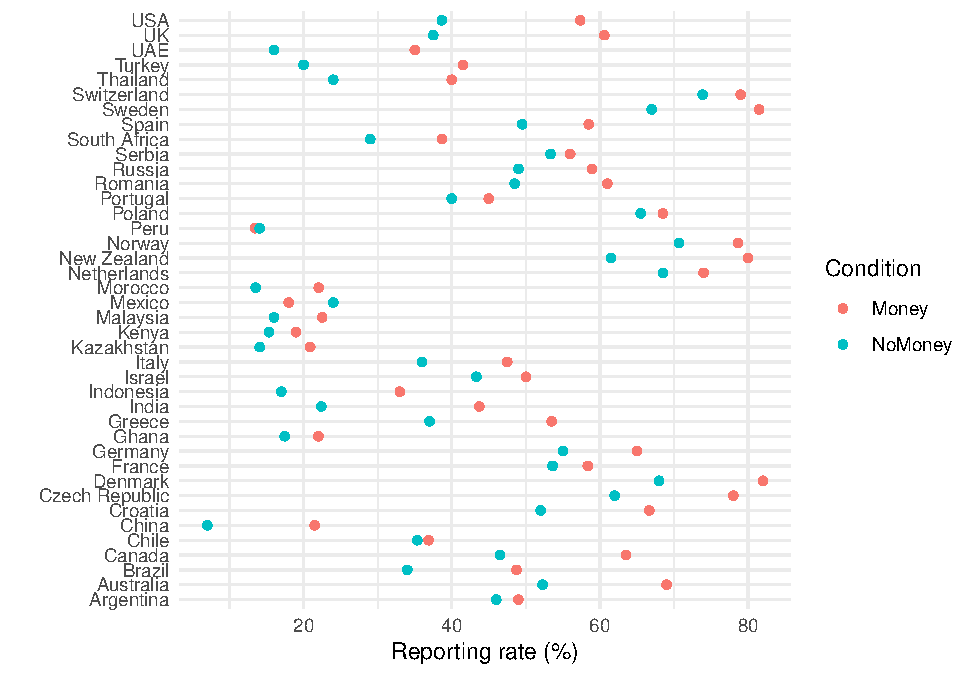
\includegraphics[width=1\linewidth]{Civic-Honesty-Replication_files/figure-latex/Figure 1-1} \caption{Share of wallets reported in the NoMoney and Money conditions, by country.}\label{fig:Figure 1-1}
\end{figure}

\begin{Shaded}
\begin{Highlighting}[]
\CommentTok{# Here's the challenging version}
\NormalTok{fig1a <-}\StringTok{ }\NormalTok{data }\OperatorTok\StringTok{ }
\StringTok{  }\KeywordTok{filter}\NormalTok{(cond }\OperatorTok\StringTok{ }\KeywordTok{c}\NormalTok{(}\DecValTok{0}\NormalTok{,}\DecValTok{1}\NormalTok{)) }\OperatorTok\StringTok{ }
\StringTok{  }\KeywordTok{mutate}\NormalTok{(}\DataTypeTok{cond =} \KeywordTok{case_when}\NormalTok{(cond }\OperatorTok{==}\StringTok{ }\DecValTok{1} \OperatorTok{~}\StringTok{ 'Money'}\NormalTok{, }
\NormalTok{                          cond }\OperatorTok{==}\StringTok{ }\DecValTok{0} \OperatorTok{~}\StringTok{ 'NoMoney'}\NormalTok{)) }\OperatorTok\StringTok{ }
\StringTok{  }\CommentTok{# compute reporting rate by country and monetary condition}
\StringTok{  }\KeywordTok{group_by}\NormalTok{(Country,}
\NormalTok{           cond) }\OperatorTok\StringTok{ }
\StringTok{  }\KeywordTok{summarize}\NormalTok{(}\DataTypeTok{pct_reported =} \KeywordTok{mean}\NormalTok{(response)) }\OperatorTok
\StringTok{  }\CommentTok{# pivot_wider to make those line segments}
\StringTok{  }\NormalTok{ungroup }\OperatorTok\StringTok{ }
\StringTok{  }\KeywordTok{pivot_wider}\NormalTok{(}\DataTypeTok{names_from =}\NormalTok{ cond, }\DataTypeTok{values_from =}\NormalTok{ pct_reported) }\OperatorTok\StringTok{ }
\StringTok{  }\CommentTok{# reorder Country by the NoMoney reporting rate }
\StringTok{  }\KeywordTok{mutate}\NormalTok{(}\DataTypeTok{Country =} \KeywordTok{fct_reorder}\NormalTok{(Country, NoMoney)) }\OperatorTok\StringTok{ }
\StringTok{  }\CommentTok{# compute label position, left of the minimum reporting rate}
\StringTok{  }\KeywordTok{mutate}\NormalTok{(}\DataTypeTok{label_position =} \KeywordTok{pmin}\NormalTok{(Money, NoMoney) }\OperatorTok{-}
\StringTok{           }\KeywordTok{nchar}\NormalTok{(}\KeywordTok{as.character}\NormalTok{(Country))}\OperatorTok{/}\FloatTok{3.5} \OperatorTok{-}\StringTok{ }\DecValTok{1}\NormalTok{) }\OperatorTok\StringTok{ }
\StringTok{  }\CommentTok{# begin ggplot}
\StringTok{  }\KeywordTok{ggplot}\NormalTok{() }\OperatorTok{+}
\StringTok{  }\KeywordTok{geom_segment}\NormalTok{(}\KeywordTok{aes}\NormalTok{(}\DataTypeTok{x=}\NormalTok{Money, }\DataTypeTok{xend=}\NormalTok{NoMoney, }\DataTypeTok{y=}\NormalTok{Country, }\DataTypeTok{yend=}\NormalTok{Country),}
               \DataTypeTok{color =} \StringTok{'gray'}\NormalTok{, }\DataTypeTok{size =} \FloatTok{0.5}\NormalTok{) }\OperatorTok{+}\StringTok{ }
\StringTok{  }\KeywordTok{geom_point}\NormalTok{(}\KeywordTok{aes}\NormalTok{(}\DataTypeTok{x=}\NormalTok{Money,}\DataTypeTok{y=}\NormalTok{Country), }\DataTypeTok{color =} \StringTok{'red'}\NormalTok{) }\OperatorTok{+}
\StringTok{  }\KeywordTok{geom_point}\NormalTok{(}\KeywordTok{aes}\NormalTok{(}\DataTypeTok{x=}\NormalTok{NoMoney,}\DataTypeTok{y=}\NormalTok{Country), }\DataTypeTok{color =} \StringTok{'#F6BE00'}\NormalTok{) }\OperatorTok{+}
\StringTok{  }\KeywordTok{geom_text}\NormalTok{(}\KeywordTok{aes}\NormalTok{(}\DataTypeTok{x=}\NormalTok{label_position, }\DataTypeTok{y=}\NormalTok{Country, }\DataTypeTok{label =}\NormalTok{ Country), }\DataTypeTok{size =} \DecValTok{2}\NormalTok{) }\OperatorTok{+}
\StringTok{  }\KeywordTok{labs}\NormalTok{(}\DataTypeTok{x =} \StringTok{'Reporting rate (%)'}\NormalTok{, }\DataTypeTok{y =} \StringTok{''}\NormalTok{, }\DataTypeTok{color =} \StringTok{'Condition'}\NormalTok{) }\OperatorTok{+}
\StringTok{  }\KeywordTok{theme_classic}\NormalTok{() }\OperatorTok{+}
\StringTok{  }\KeywordTok{theme}\NormalTok{(}\DataTypeTok{axis.text.y =} \KeywordTok{element_blank}\NormalTok{(),}
        \DataTypeTok{axis.ticks.y =} \KeywordTok{element_blank}\NormalTok{(),}
        \DataTypeTok{axis.line.y =} \KeywordTok{element_blank}\NormalTok{())}

\NormalTok{fig1a}
\end{Highlighting}
\end{Shaded}

\begin{figure}[p]
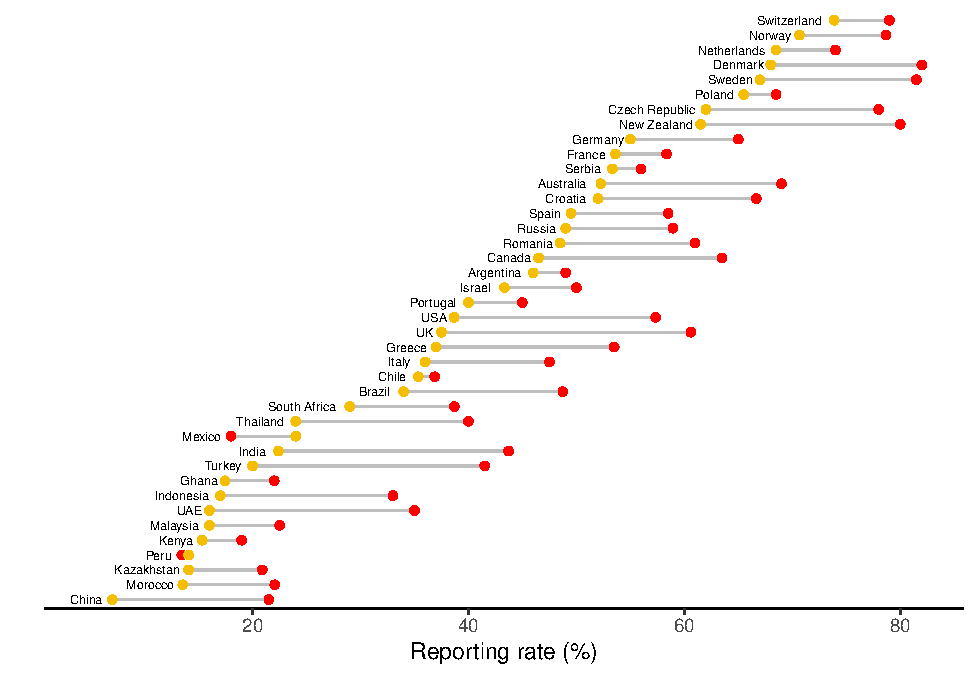
\includegraphics[width=1\linewidth]{Civic-Honesty-Replication_files/figure-latex/Figure 1-2} \caption{Share of wallets reported in the NoMoney and Money conditions, by country.}\label{fig:Figure 1-2}
\end{figure}

\hypertarget{replicating-figure-2}{%
\subsection{Replicating Figure 2}\label{replicating-figure-2}}

Now replicate Figure 2. To do so, we need to perform the following
steps:

\begin{itemize}
\tightlist
\item
  Keep only the data from Poland, the United Kingdom, and the United
  States
\item
  Keep only the NoMoney, Money, and BigMoney conditions
\item
  Recode the \texttt{cond} variable as ``NoMoney'', ``Money'' and
  ``BigMoney''
\item
  Compute the average response rate, grouped by country and condition.
\item
  Plot a scatter with condition on the x-axis, reporting rate on the
  y-axis, and colored by country.
\item
  Add a \texttt{geom\_line()} layer with the same aesthetics (also
  include \texttt{group\ =\ Country} as an aesthetic).
\end{itemize}

As an extra challenge, you can do any combination of the following:

\begin{itemize}
\tightlist
\item
  Use original colors from the paper
\item
  Use the ggplot theme that best matches the theme from the paper
\item
  Reorder the \texttt{cond} variable so it appears in the same order as
  the original Figure 2
\item
  Include country labels as in the paper with \texttt{geom\_dl()} from
  the \texttt{directlabels} package, and remove the legend
\end{itemize}

\begin{Shaded}
\begin{Highlighting}[]
\CommentTok{# Basic version}
\NormalTok{data }\OperatorTok\StringTok{ }
\StringTok{  }\KeywordTok{filter}\NormalTok{(Country }\OperatorTok\StringTok{ }\KeywordTok{c}\NormalTok{(}\StringTok{'Poland'}\NormalTok{, }\StringTok{'UK'}\NormalTok{, }\StringTok{'USA'}\NormalTok{),}
\NormalTok{         cond }\OperatorTok\StringTok{ }\DecValTok{0}\OperatorTok{:}\DecValTok{2}\NormalTok{) }\OperatorTok\StringTok{ }
\StringTok{  }\KeywordTok{mutate}\NormalTok{(}\DataTypeTok{cond =} \KeywordTok{case_when}\NormalTok{(cond }\OperatorTok{==}\StringTok{ }\DecValTok{0} \OperatorTok{~}\StringTok{ 'NoMoney'}\NormalTok{,}
\NormalTok{                          cond }\OperatorTok{==}\StringTok{ }\DecValTok{1} \OperatorTok{~}\StringTok{ 'Money'}\NormalTok{,}
\NormalTok{                          cond }\OperatorTok{==}\StringTok{ }\DecValTok{2} \OperatorTok{~}\StringTok{ 'BigMoney'}\NormalTok{)) }\OperatorTok\StringTok{ }
\StringTok{  }\KeywordTok{group_by}\NormalTok{(Country, cond) }\OperatorTok\StringTok{ }
\StringTok{  }\KeywordTok{summarize}\NormalTok{(}\DataTypeTok{reporting_rate =} \KeywordTok{mean}\NormalTok{(response)) }\OperatorTok\StringTok{ }
\StringTok{  }\KeywordTok{ggplot}\NormalTok{() }\OperatorTok{+}\StringTok{ }
\StringTok{  }\KeywordTok{geom_point}\NormalTok{(}\DataTypeTok{mapping =} \KeywordTok{aes}\NormalTok{(}\DataTypeTok{x =}\NormalTok{ cond, }\DataTypeTok{y =}\NormalTok{ reporting_rate,}
                           \DataTypeTok{color =}\NormalTok{ Country)) }\OperatorTok{+}\StringTok{ }
\StringTok{  }\KeywordTok{geom_line}\NormalTok{(}\DataTypeTok{mapping =} \KeywordTok{aes}\NormalTok{(}\DataTypeTok{x =}\NormalTok{ cond, }\DataTypeTok{y =}\NormalTok{ reporting_rate,}
                          \DataTypeTok{group =}\NormalTok{ Country, }\DataTypeTok{color =}\NormalTok{ Country)) }\OperatorTok{+}\StringTok{ }
\StringTok{  }\KeywordTok{labs}\NormalTok{(}\DataTypeTok{x =} \StringTok{''}\NormalTok{, }\DataTypeTok{y =} \StringTok{'Reporting Rate (%)'}\NormalTok{) }\OperatorTok{+}
\StringTok{  }\KeywordTok{theme_classic}\NormalTok{()}
\end{Highlighting}
\end{Shaded}

\begin{figure}[p]
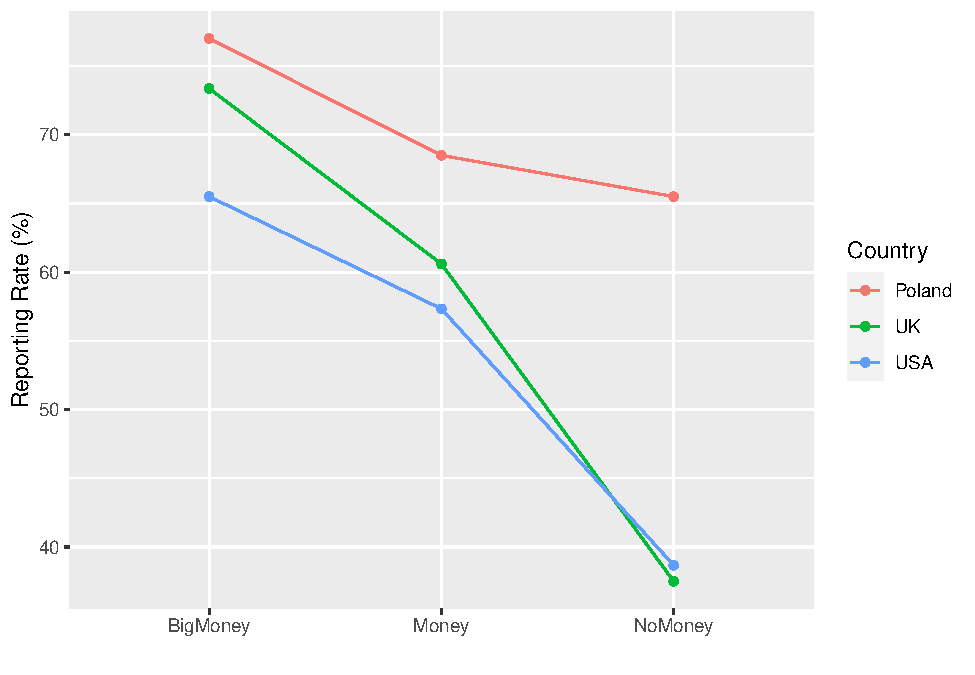
\includegraphics[width=1\linewidth]{Civic-Honesty-Replication_files/figure-latex/Figure 2-1} \caption{Reporting rates as a function of monetary stakes}\label{fig:Figure 2-1}
\end{figure}

\begin{Shaded}
\begin{Highlighting}[]
\KeywordTok{library}\NormalTok{(directlabels)}

\CommentTok{# Harder version}
\NormalTok{data }\OperatorTok\StringTok{ }
\StringTok{  }\KeywordTok{filter}\NormalTok{(Country }\OperatorTok\StringTok{ }\KeywordTok{c}\NormalTok{(}\StringTok{'Poland'}\NormalTok{, }\StringTok{'UK'}\NormalTok{, }\StringTok{'USA'}\NormalTok{),}
\NormalTok{         cond }\OperatorTok\StringTok{ }\DecValTok{0}\OperatorTok{:}\DecValTok{2}\NormalTok{) }\OperatorTok\StringTok{ }
\StringTok{  }\KeywordTok{mutate}\NormalTok{(}\DataTypeTok{Country =} \KeywordTok{case_when}\NormalTok{(Country }\OperatorTok{==}\StringTok{ 'UK'} \OperatorTok{~}\StringTok{ 'United Kingdom'}\NormalTok{,}
\NormalTok{                             Country }\OperatorTok{==}\StringTok{ 'USA'} \OperatorTok{~}\StringTok{ 'United States'}\NormalTok{,}
                             \OtherTok{TRUE} \OperatorTok{~}\StringTok{ }\NormalTok{Country),}
         \DataTypeTok{cond =} \KeywordTok{case_when}\NormalTok{(cond }\OperatorTok{==}\StringTok{ }\DecValTok{0} \OperatorTok{~}\StringTok{ 'NoMoney'}\NormalTok{,}
\NormalTok{                          cond }\OperatorTok{==}\StringTok{ }\DecValTok{1} \OperatorTok{~}\StringTok{ 'Money'}\NormalTok{,}
\NormalTok{                          cond }\OperatorTok{==}\StringTok{ }\DecValTok{2} \OperatorTok{~}\StringTok{ 'BigMoney'}\NormalTok{)) }\OperatorTok\StringTok{ }
\StringTok{  }\KeywordTok{group_by}\NormalTok{(Country, cond) }\OperatorTok\StringTok{ }
\StringTok{  }\KeywordTok{summarize}\NormalTok{(}\DataTypeTok{reporting_rate =} \KeywordTok{mean}\NormalTok{(response)) }\OperatorTok\StringTok{ }
\StringTok{  }\KeywordTok{mutate}\NormalTok{(}\DataTypeTok{cond =} \KeywordTok{factor}\NormalTok{(cond, }\DataTypeTok{levels =} \KeywordTok{c}\NormalTok{(}\StringTok{'NoMoney'}\NormalTok{, }\StringTok{'Money'}\NormalTok{, }\StringTok{'BigMoney'}\NormalTok{))) }\OperatorTok\StringTok{ }
\StringTok{  }\KeywordTok{ggplot}\NormalTok{() }\OperatorTok{+}\StringTok{ }
\StringTok{  }\KeywordTok{geom_point}\NormalTok{(}\DataTypeTok{mapping =} \KeywordTok{aes}\NormalTok{(}\DataTypeTok{x =}\NormalTok{ cond, }\DataTypeTok{y =}\NormalTok{ reporting_rate,}
                           \DataTypeTok{color =}\NormalTok{ Country)) }\OperatorTok{+}\StringTok{ }
\StringTok{  }\KeywordTok{geom_line}\NormalTok{(}\DataTypeTok{mapping =} \KeywordTok{aes}\NormalTok{(}\DataTypeTok{x =}\NormalTok{ cond, }\DataTypeTok{y =}\NormalTok{ reporting_rate,}
                          \DataTypeTok{group =}\NormalTok{ Country, }\DataTypeTok{color =}\NormalTok{ Country)) }\OperatorTok{+}\StringTok{ }
\StringTok{  }\KeywordTok{geom_dl}\NormalTok{(}\DataTypeTok{mapping =} \KeywordTok{aes}\NormalTok{(}\DataTypeTok{x=}\NormalTok{cond, }\DataTypeTok{y=}\NormalTok{reporting_rate, }\DataTypeTok{label =}\NormalTok{ Country),}
          \DataTypeTok{method =} \KeywordTok{list}\NormalTok{(}\KeywordTok{dl.trans}\NormalTok{(}\DataTypeTok{x =}\NormalTok{ x }\OperatorTok{+}\StringTok{ }\FloatTok{0.2}\NormalTok{), }\StringTok{'last.points'}\NormalTok{, }\DataTypeTok{cex =} \FloatTok{0.75}\NormalTok{)) }\OperatorTok{+}
\StringTok{  }\KeywordTok{scale_color_manual}\NormalTok{(}\DataTypeTok{values =} \KeywordTok{c}\NormalTok{(}\StringTok{'#8b1b1e'}\NormalTok{, }\StringTok{'#f23524'}\NormalTok{, }\StringTok{'#f98f1c'}\NormalTok{)) }\OperatorTok{+}
\StringTok{  }\KeywordTok{labs}\NormalTok{(}\DataTypeTok{x =} \StringTok{''}\NormalTok{, }\DataTypeTok{y =} \StringTok{'Reporting Rate (%)'}\NormalTok{) }\OperatorTok{+}
\StringTok{  }\KeywordTok{theme_classic}\NormalTok{() }\OperatorTok{+}
\StringTok{  }\KeywordTok{theme}\NormalTok{(}\DataTypeTok{legend.position =} \StringTok{'none'}\NormalTok{)}
\end{Highlighting}
\end{Shaded}

\begin{figure}[p]
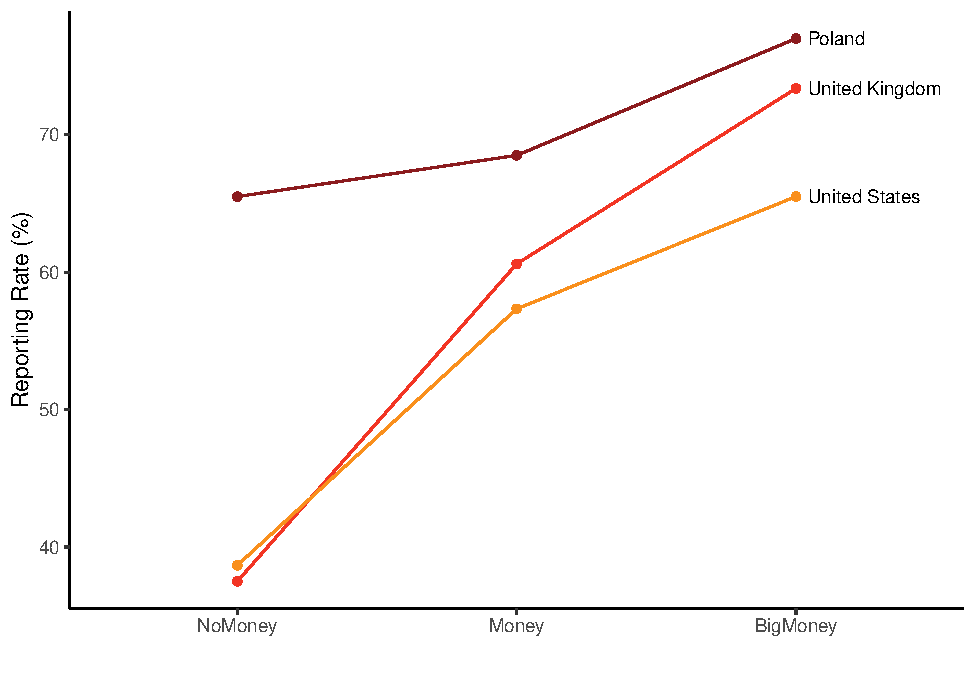
\includegraphics[width=1\linewidth]{Civic-Honesty-Replication_files/figure-latex/Figure 2-2} \caption{Reporting rates as a function of monetary stakes}\label{fig:Figure 2-2}
\end{figure}

\hypertarget{references}{%
\section*{References}\label{references}}
\addcontentsline{toc}{section}{References}

\hypertarget{refs}{}
\leavevmode\hypertarget{ref-cohnCivicHonestyGlobe2019}{}%
Cohn, Alain, Michel André Maréchal, David Tannenbaum, and Christian
Lukas Zünd. 2019. ``Civic Honesty Around the Globe.'' \emph{Science} 365
(6448): 70--73. \url{https://doi.org/10.1126/science.aau8712}.






\end{document}
